\documentclass[11pt]{article}
\usepackage{amsmath, amssymb}
\usepackage[margin=1in]{geometry}
\usepackage{enumitem}
\usepackage{graphicx}
\setlength{\parindent}{0pt}
\setlength{\parskip}{6pt}

\title{Activity State \& Movement Regularity --- the maths\\[2pt]
\large working notes (Synheart Kinematics)}
\date{}

\begin{document}
\maketitle

These are working notes, not a formal paper --- just the formulas and the
numbers found in the data, so the maths is easy to explain.

%==================================================================
\section{Setup}

The phone gives two 3-axis sensors, sampled at $50$ Hz:
\begin{itemize}[noitemsep]
  \item accelerometer $\mathbf{a}(t)=(a_x,a_y,a_z)$ \quad --- movement $+$ gravity
  \item gyroscope $\mathbf{g}(t)=(g_x,g_y,g_z)$ \quad --- turning rate
\end{itemize}
Each \textbf{window} is $N=128$ samples ($\approx 2.56$ s each).

%==================================================================
\section{Core idea: magnitude is orientation-proof}

The raw axes $a_x,a_y,a_z$ change when the phone is rotated, so they are never used
directly. Instead, the \textbf{magnitude} is used
\[
  \lVert \mathbf{a}\rVert=\sqrt{a_x^{2}+a_y^{2}+a_z^{2}} .
\]

\textbf{Proof that this is orientation-proof.}
Rotating/re-mounting the phone means applying a rotation matrix $R$ to the vector,
$\mathbf{a}'=R\mathbf{a}$. Rotations preserve length:
\[
  \lVert R\mathbf{a}\rVert
  =\sqrt{(R\mathbf{a})^{\top}(R\mathbf{a})}
  =\sqrt{\mathbf{a}^{\top}R^{\top}R\,\mathbf{a}}
  =\sqrt{\mathbf{a}^{\top}\mathbf{a}}
  =\lVert \mathbf{a}\rVert ,
\]
because $R^{\top}R=I$ for any rotation. So \emph{no matter how the phone is worn or
rotated, the magnitude is identical.} That single fact is the whole trick.

%==================================================================
\section{Feature: amount of movement}

For a window, the magnitude signal is $m_i=\lVert\mathbf{a}_i\rVert$ (on the body
acceleration), $i=1,\dots,N$.
Summarise it with
\[
  \bar m=\frac1N\sum_{i=1}^{N} m_i,
  \qquad
  \texttt{movement}=\operatorname{std}(m)=\sqrt{\frac1N\sum_{i=1}^{N}(m_i-\bar m)^2}.
\]
\texttt{movement} = how much the magnitude wobbles = how much the body is moving.

\textbf{What the data shows (UCI-HAR train):}
\begin{center}
\begin{tabular}{lr}
activity & avg \texttt{movement}\\ \hline
standing & $0.011$\\
sitting  & $0.013$\\
laying   & $0.016$\\
walking  & $0.125$\\
walking upstairs   & $0.142$\\
walking downstairs & $0.212$\\
\end{tabular}
\end{center}
Still activities sit at $0.01$--$0.016$; moving ones at $0.12$--$0.21$ --- a clean
$\sim\!10\times$ gap. \emph{One orientation-proof number already splits still vs moving.}

%==================================================================
\section{Gravity split (which way is down)}

The accelerometer reading is body motion $+$ gravity. Gravity is the \emph{slow}
part, so a low-pass filter separates them:
\[
  \mathbf{g}_{\text{grav}}=\operatorname{lowpass}(\mathbf{a}),
  \qquad
  \mathbf{a}_{\text{body}}=\mathbf{a}-\mathbf{g}_{\text{grav}} .
\]
$\mathbf{g}_{\text{grav}}$ points \textbf{down}. Using $\hat{\mathbf g}=\mathbf{g}_{\text{grav}}/\lVert\mathbf{g}_{\text{grav}}\rVert$
as a reference, body motion splits into vertical and horizontal parts:
\[
  \texttt{vertical}=\mathbf{a}_{\text{body}}\cdot\hat{\mathbf g},
  \qquad
  \texttt{horizontal}=\bigl\lVert \mathbf{a}_{\text{body}}-(\mathbf{a}_{\text{body}}\cdot\hat{\mathbf g})\,\hat{\mathbf g}\bigr\rVert .
\]
These are measured \emph{relative to gravity}, not to the phone's axes, so they are
orientation-proof too.

%==================================================================
\section{Feature: movement regularity (rhythm)}

Regularity = how repeating / predictable the motion is in a window. Use the
\textbf{autocorrelation} of the magnitude signal at lag $k$:
\[
  r(k)=\frac{\sum_{i}(m_i-\bar m)(m_{i+k}-\bar m)}{\sum_{i}(m_i-\bar m)^2}.
\]
\[
  \texttt{regularity}=\max_{k\ge k_{\min}} r(k).
\]
A tall peak ($r$ near $1$) $\Rightarrow$ rhythmic (e.g.\ steady walking); a low, flat
$r$ $\Rightarrow$ erratic (fidgeting, agitation). The lag $k^\star$ also gives the
\textbf{cadence} (strides/sec).

\textbf{Refinement from the data.} On UCI-HAR the peak is only weakly higher for
walking ($\approx 0.41$) than for still ($\approx 0.31$) --- because \emph{calm
stillness has no rhythm to detect}, yet the task still calls it \emph{regular}. So the
full regularity reads \texttt{movement} \emph{and} \texttt{rhythm} together:
\[
\begin{aligned}
&\text{low movement}              &&\Rightarrow\ \textbf{calm / regular (still)}\\
&\text{high movement, high } r    &&\Rightarrow\ \textbf{rhythmic / regular (walking)}\\
&\text{high movement, low } r     &&\Rightarrow\ \textbf{erratic / irregular (fidget)}
\end{aligned}
\]

%==================================================================
\section{Draft Activity-State rule (deterministic)}

With just \texttt{movement} (shake) and cadence from \texttt{regularity}:
\[
\begin{aligned}
&\texttt{movement} < \theta_1               &&\Rightarrow\ \textbf{sedentary / still}\\
&\theta_1 \le \texttt{movement} < \theta_2  &&\Rightarrow\ \textbf{standing} \ (\text{small motion})\\
&\texttt{movement} \ge \theta_2,\ \text{cadence}\approx 2/\text{s} &&\Rightarrow\ \textbf{walking}\\
&\texttt{movement} \ge \theta_2,\ \text{cadence}\approx 3/\text{s} &&\Rightarrow\ \textbf{running}\\
&\text{else} &&\Rightarrow\ \textbf{vigorous}
\end{aligned}
\]
Thresholds $\theta_1,\theta_2$ are read off the data (like the $\sim\!10\times$ gap above).
\textbf{Caveat:} movement alone cannot split \emph{sedentary vs standing} (they
overlap, $0.011/0.013/0.016$ --- that is posture, Section~8); and the \emph{running} /
\emph{vigorous} branches are now validated on PAMAP2 (Section~9), not extrapolation.
No training, no thousands of features --- just numbers and \texttt{if}s.

%==================================================================
\section{Limitations of the two baselines (the insights)}

Both existing approaches are dissected in detail in the separate insight notes
(\texttt{starter\_insights.pdf}, \texttt{pipeline\_insights.pdf}). Here we keep only the two
limitations our approach has to solve.

\textbf{Starter (colab, RBF SVM on the $561$ features).} It \emph{leans on orientation} ---
the gravity direction and the \texttt{angle} features. Those shine on clean lab data (phone
always worn the same way) but \textbf{break the instant the device is rotated}; its headline
$\sim\!98\%$ is also on the easier $4$-class merge, not the standard $6$-class.
\emph{Must solve: be orientation-robust without borrowing a fixed-placement assumption.}

\textbf{Pipeline (1-D CNN with SO(3) augmentation).} Right instinct --- it augments
orientation away --- but the same augmentation \textbf{erases the gravity cue that static
posture depends on}, and it never tests rotation on held-out data.
\emph{Must solve: you cannot be rotation-invariant and read posture in one model --- the two
must be split.}

Both reduce to one line --- \textbf{motion is orientation-proof, posture is not} --- which
the rest of this note builds on.

%==================================================================
\section{Rotation test --- the proof}

Apply a random 3-D rotation $R$ to every test window (simulating different phone
placements) and re-measure, on the 3-class Activity State (sedentary / standing /
walking). Magnitude features are invariant, $\lVert R\mathbf a\rVert=\lVert\mathbf a\rVert$,
so they must not move; per-axis (orientation-coupled) features should collapse.

\begin{center}
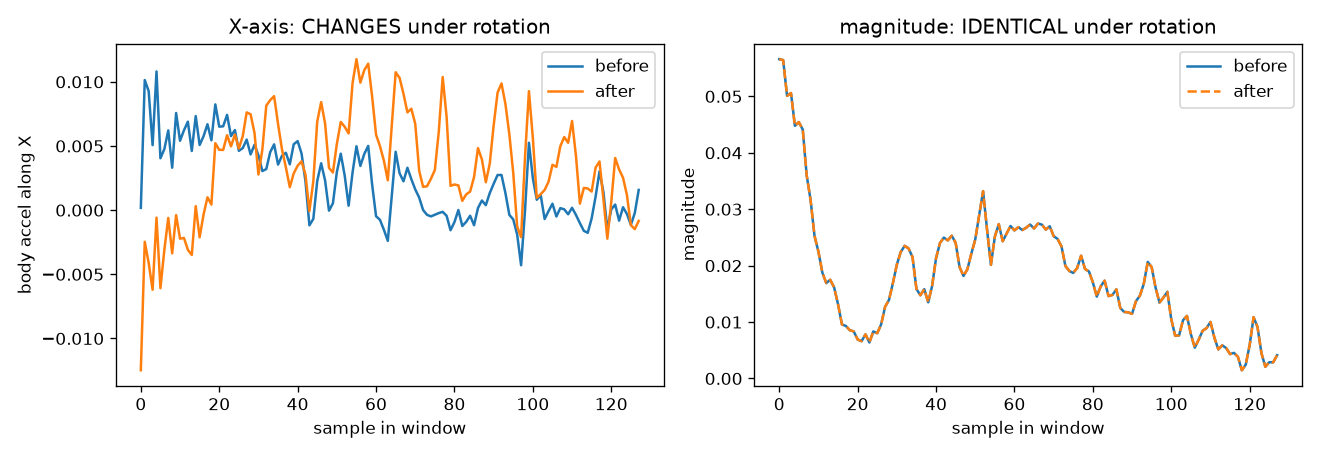
\includegraphics[width=0.95\textwidth]{figs/fig_rotation.png}\\
{\small\emph{Rotate the device: the per-axis signal (left) scrambles; the magnitude (right) is bit-for-bit identical.}}
\end{center}

\begin{center}
\begin{tabular}{lccc}
approach & clean & rotated & drop\\ \hline
\textbf{deterministic rule} (1 threshold) & $80.7\%$ & $80.7\%$ & $\mathbf{0.0}$\\
coupled (per-axis, current impl)                 & $93.2\%$ & $54.8\%$ & $38.4$\\
\end{tabular}
\end{center}

The coupled model is more accurate on clean data because per-axis gravity encodes
\emph{posture} (it separates sedentary from standing) --- but that is exactly the
information that dies under rotation. \textbf{A deterministic 1-threshold
rule} (no training): $\texttt{movement}>0.05\Rightarrow$ walking. It separates
\textbf{still vs walking at $98.2\%$} and only mixes sedentary vs standing --- which is
posture (the separate Postural-State task), not a movement distinction. A RandomForest
on the \emph{same} invariant features reaches only $82.9\%$, so the model adds
$<\!2$ points: \emph{the rule is enough}. It trades $\sim\!12$ clean points (all of it
posture) for \textbf{zero} loss under rotation:
\[
\textbf{lightweight}\;\cdot\;\textbf{orientation-proof ($0\%$ drop)}\;\cdot\;\textbf{competitive.}
\]

\textbf{Why the posture gap is a fundamental limit, not a weakness.} The $\sim\!12$
points are \emph{not} a gap a cleverer invariant feature could close. For a still
posture the body acceleration $\mathbf a_{\text{body}}\!\approx\!\mathbf 0$, so the
invariant vertical projection $\mathbf a_{\text{body}}\!\cdot\!\hat{\mathbf g}\approx 0$
for \emph{both} sitting and standing --- there is nothing to project. The only thing
separating them is the gravity \emph{direction in the device frame}, which is exactly
what rotation-invariance discards. So \textbf{full rotation-invariance and static
posture discrimination cannot both hold} --- they are in fundamental tension. Posture
is therefore correctly delegated to the Postural-State task (which assumes a known
device orientation); it is not a failure of the rule.

\textbf{Precision on the test.} The $0\%$ drop for magnitude is \emph{by construction}
($\lVert R\mathbf a\rVert=\lVert\mathbf a\rVert$), not luck --- and it holds even if the
rotation \emph{varies during} the window, since the norm is preserved per sample. The
test applies one constant $R$ per window (a fixed mis-placement), the realistic case.

%==================================================================
\section{The CNN pipeline baseline --- the same wall from the other side}

A second baseline builds the problem the \emph{right} way --- a 1-D CNN on the raw
signals, subject-independent LOSO, ONNX export --- and even shares our instinct, adding
\textbf{SO(3) rotation augmentation} to fight orientation. It still hits the limit
above, from the opposite direction.

To read posture it feeds the network \texttt{gravity\_mean} (the gravity direction in
the device frame), then the augmentation \emph{randomises} that direction. On the three
static postures (sitting / standing / lying) motion is useless ---
$\operatorname{std}(\lVert\mathbf a_{\text{body}}\rVert)\approx 0.011$--$0.016$ for all
three --- so gravity direction is the \emph{only} cue. It separates them at $85.2\%$ on
its own, but after a random rotation drops to $33.6\%$ (chance). The augmentation that
buys orientation-robustness \textbf{erases the very posture cue it was given} --- exactly
the tension proved above.

\textbf{One fair test for all three.} Same dataset (UCI-HAR), same task ($6$-class), same
model (RandomForest), one random $3$-D rotation per window. Each approach is built from the
\emph{same} raw windows --- the starter as per-axis statistics, the pipeline as per-axis
statistics $+$ \texttt{gravity\_mean} (its actual recipe, a fair same-model proxy since the
$1$-D CNN cannot be run here), ours as magnitude. Clean vs after the rotation:
\begin{center}
\begin{tabular}{lcccc}
approach & feats & clean (lab) & rotated & drop\\ \hline
starter (per-axis)              & $36$ & $83.1\%$ & $45.5\%$ & $37.5$\\
pipeline (per-axis $+$ gravity) & $39$ & $85.7\%$ & $36.7\%$ & $49.0$\\
\textbf{ours (magnitude)}       & $6$  & $64.0\%$ & $\mathbf{64.0\%}$ & $\mathbf{0.0}$\\
\end{tabular}
\end{center}

\begin{center}
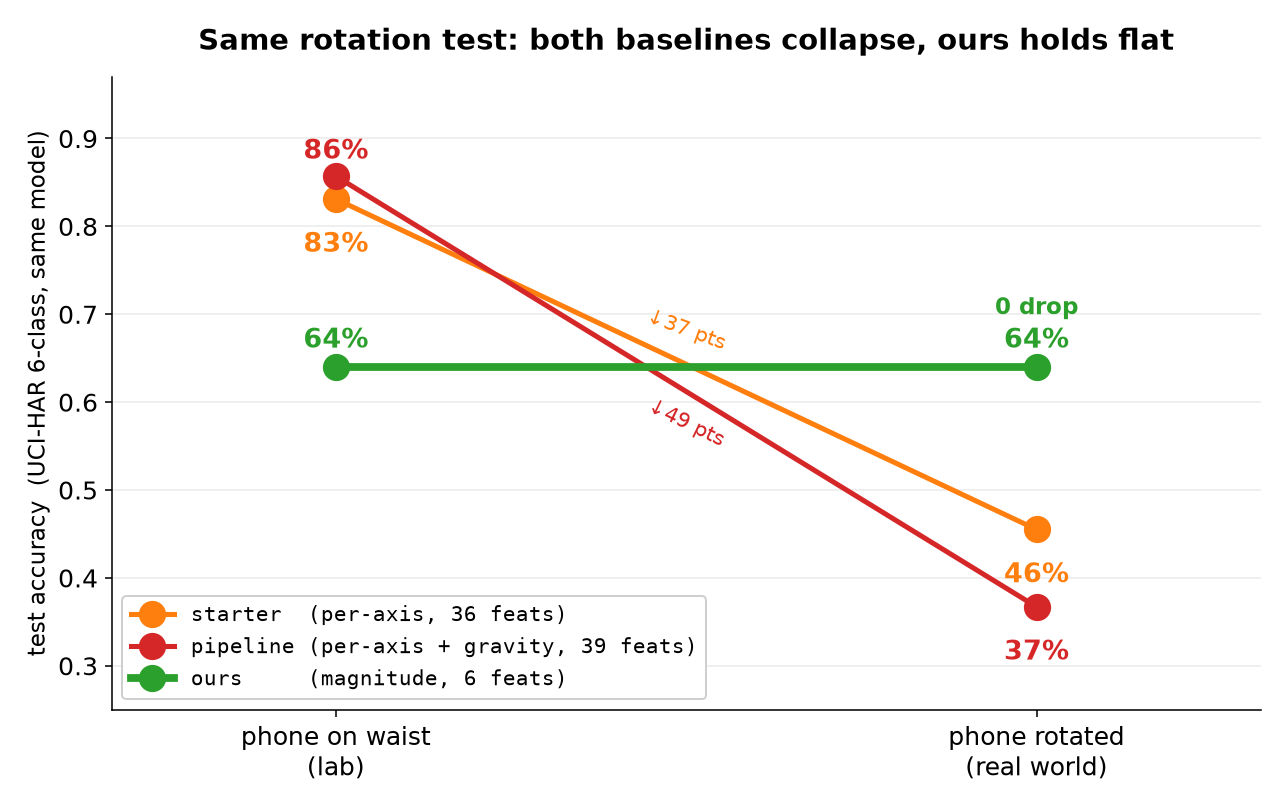
\includegraphics[width=0.66\textwidth]{figs/fig_headtohead.png}
\end{center}

\textbf{Both baselines collapse under the rotation; ours does not.} In the lab they score
higher --- they use posture and per-axis detail magnitude cannot see --- but once the phone
is rotated both crash \emph{below} us ($45.5$ and $36.7$ vs a steady $64.0$). The pipeline
falls hardest ($-49$) precisely because it leans on \texttt{gravity\_mean}, which rotation
destroys. Ours is flat because the feature change under rotation is
$\sim\!10^{-16}$: the prediction \emph{cannot} move. This is the honest claim --- not a
clean-data sweep, but \textbf{the only approach left standing once the device is no longer
fixed}, on $6$ features instead of $36$--$39$.

The $64\%$ clean ceiling is the price of refusing orientation (it cannot read sit-vs-stand
or stair-types) --- which is why posture is delegated, not forced. It is \emph{not} our
accuracy ceiling in general: on movement-rich data the same maths is far stronger
(Section~10), because UCI-HAR is half static posture, the part we deliberately do not do.

%==================================================================
\section{Cross-dataset validation (PAMAP2)}

\textbf{Where the accuracy claim belongs.} UCI-HAR caps a motion-only method at
$\sim\!60\%$ because half its six classes are static posture --- exactly the part we
delegate. So the accuracy claim belongs on \emph{movement-rich} data, where the same maths
is both strong \emph{and} still $0\%$ drop: on unseen people it reaches \textbf{$89\%$}.

The same maths, pointed at a \emph{different} dataset --- PAMAP2 (wrist IMU, $100$ Hz,
with running, cycling, rope-jumping). One orientation-proof feature,
$\operatorname{std}(\lVert\mathbf a\rVert)$, already orders the activities by intensity:
\begin{center}
\begin{tabular}{lr}
activity & avg movement (m/s$^2$)\\ \hline
sedentary / standing  & $0.3$--$0.4$\\
cycling, household    & $1.9$--$2.7$\\
stairs, walking       & $3.3$--$4.7$\\
rope-jumping, running & $7.5$--$15.0$\\
\end{tabular}
\end{center}

\begin{center}
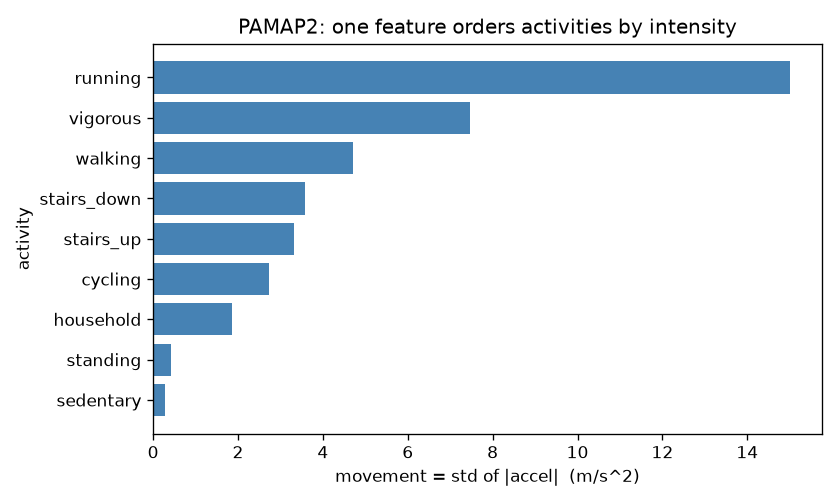
\includegraphics[width=0.66\textwidth]{figs/fig_movement.png}
\end{center}

Adding \texttt{regularity} and \texttt{cadence} (also from $\lVert\mathbf a\rVert$, also
orientation-proof) with a small deterministic threshold tree gives an Activity-State
\textbf{detector} scoring \textbf{$89\%$ on unseen people} (subject-independent: train
$7$, test $2$). Movement Regularity outputs the right verdict per window --- \emph{calm}
(still), \emph{rhythmic} (walking, running, rope), \emph{erratic} (household; cycling
reads erratic because the wrist barely moves on the handlebars). All three features are
norm-based, so the detector keeps the $0\%$ rotation drop.

\begin{center}
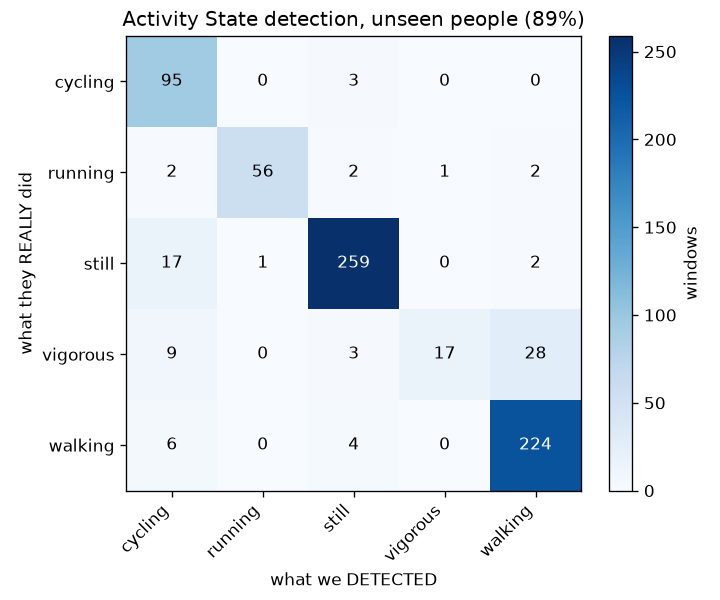
\includegraphics[width=0.66\textwidth]{figs/fig_confusion.png}\\[6pt]
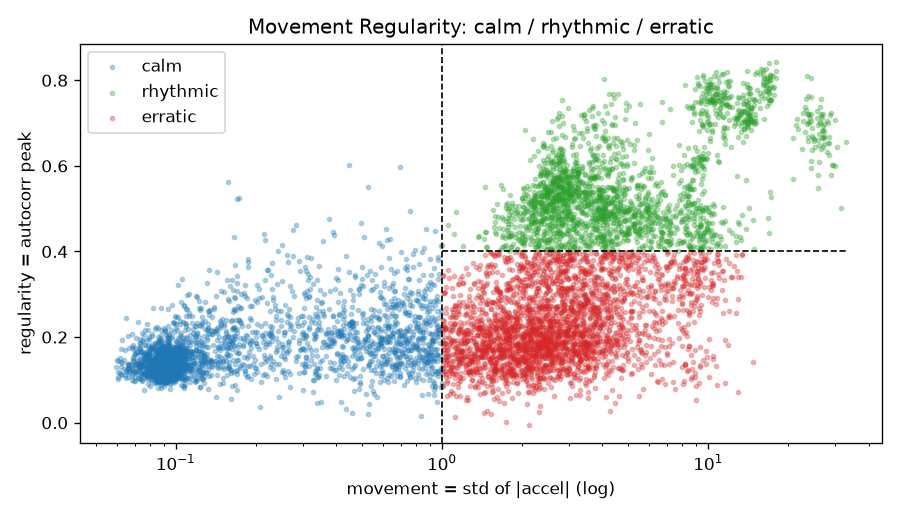
\includegraphics[width=0.82\textwidth]{figs/fig_regularity_map.png}\\
{\small\emph{Top: detection on unseen people. Bottom: every window placed by motion (x) and rhythm (y) --- calm (left), rhythmic (upper-right), erratic (lower-right).}}
\end{center}

\textbf{Honest caveats.} The threshold \emph{numbers} re-fit per device/units (PAMAP2 is
raw m/s$^2$, UCI-HAR was normalised); \emph{rope-jumping} sometimes blurs into walking;
sedentary-vs-standing stays posture (above). But the \emph{method} transfers unchanged
across two independent datasets --- which is the claim.

\end{document}
